% allgem. Dokumentenformat
\documentclass[a4paper,12pt,headsepline]{scrartcl}

% weitere Pakete
% Grafiken aus PNG Dateien einbinden
\usepackage{graphicx}

% Normabstand bei Einheiten
\usepackage{siunitx}

% Deutsche Sonderzeichen benutzen 
\usepackage{ngerman}

% deutsche Silbentrennung
\usepackage[ngerman]{babel}

% Eurozeichen einbinden
\usepackage[right]{eurosym}

% Umlaute unter UTF8 nutzen
\usepackage[utf8]{inputenc}

% Zeichenencoding
\usepackage[T1]{fontenc}

\usepackage{lmodern}
\usepackage{fix-cm}

% floatende Bilder ermöglichen
%\usepackage{floatflt}

% mehrseitige Tabellen ermöglichen
\usepackage{longtable}

% Unterstützung für Schriftarten
%\newcommand{\changefont}[3]{ 
%\fontfamily{#1} \fontseries{#2} \fontshape{#3} \selectfont}

% Packet für Seitenrandabständex und Einstellung für Seitenränder
\usepackage{geometry}
\geometry{left=3.5cm, right=2cm, top=2.5cm, bottom=2cm}

% Paket für Boxen im Text
\usepackage{fancybox}

% bricht lange URLs "schoen" um
\usepackage[hyphens,obeyspaces,spaces]{url}

% Paket für Textfarben
\usepackage{color}

% Mathematische Symbole importieren
\usepackage{amssymb}

% auf jeder Seite eine Überschrift (alt, zentriert)
%\pagestyle{headings}

% erzeugt Inhaltsverzeichnis mit Querverweisen zu den Kapiteln (PDF Version)
\usepackage[bookmarksnumbered,pdftitle={Hausarbeit im Seminar 21817 „IT-Sicherheit“},hyperfootnotes=true]{hyperref} 
%\hypersetup{colorlinks, citecolor=red, linkcolor=blue, urlcolor=black}
\hypersetup{colorlinks, citecolor=black, linkcolor= black, urlcolor=black}

% neue Kopfzeilen mit fancypaket
\usepackage{fancyhdr} %Paket laden
\pagestyle{fancy} %eigener Seitenstil
\fancyhf{} %alle Kopf- und Fußzeilenfelder bereinigen
\fancyhead[L]{} %Kopfzeile links
\fancyhead[C]{} %zentrierte Kopfzeile
\fancyhead[R]{\thepage} %Kopfzeile rechts
\renewcommand{\headrulewidth}{0.4pt} %obere Trennlinie
%\fancyfoot[C]{\thepage} %Seitennummer
%\renewcommand{\footrulewidth}{0.4pt} %untere Trennlinie

% für Tabellen
\usepackage{array}

% Runde Klammern für Zitate
%\usepackage[numbers,round]{natbib}

% Festlegung Art der Zitierung - Havardmethode: Abkuerzung Autor + Jahr
\bibliographystyle{alphadin}

% Schaltet den zusätzlichen Zwischenraum ab, den LaTeX normalerweise nach einem Satzzeichen einfügt.
\frenchspacing

% Paket für Zeilenabstand
\usepackage{setspace}

% für Bildbezeichner
\usepackage{capt-of}

% für Stichwortverzeichnis
\usepackage{makeidx}

% für Listings
\usepackage{listings}
\lstset{numbers=left, numberstyle=\tiny, numbersep=5pt, keywordstyle=\color{black}\bfseries, stringstyle=\ttfamily,showstringspaces=false,basicstyle=\footnotesize,captionpos=b}
\lstset{language=perl}

% Indexerstellung
\makeindex

% Abkürzungsverzeichnis
\usepackage[german]{nomencl}
\let\abbrev\nomenclature

% Abkürzungsverzeichnis LiveTex Version
\renewcommand{\nomname}{Abkürzungsverzeichnis}
\setlength{\nomlabelwidth}{.25\hsize}
\renewcommand{\nomlabel}[1]{#1 \dotfill}
\setlength{\nomitemsep}{-\parsep}
\makenomenclature
%\makeglossary

% Abkürzungsverzeichnis TeTEX Version
\usepackage[german]{nomencl}
\makenomenclature
%\makeglossary
\renewcommand{\nomname}{Abkürzungsverzeichnis}
\setlength{\nomlabelwidth}{.25\hsize}
\renewcommand{\nomlabel}[1]{#1 \dotfill}
\setlength{\nomitemsep}{-\parsep}

% Disable single lines at the start of a paragraph (Schusterjungen)
\clubpenalty = 10000
% Disable single lines at the end of a paragraph (Hurenkinder)
\widowpenalty = 10000
\displaywidowpenalty = 10000

\begin{document}
% hier werden die Trennvorschläge inkludiert
%hier müssen alle Wörter rein, welche Latex von sich auch nicht korrekt trennt bzw. bei denen man die genaue Trennung vorgeben möchte
\hyphenation{
Film-pro-du-zen-ten
Lux-em-burg
Soft-ware-bau-steins
zeit-in-ten-siv
In-jec-tion-Sch-wach-stel-len
}


%Schriftart Helvetica
%\changefont{phv}{m}{n}

% Leere Seite am Anfang
%~ \newpage
\thispagestyle{empty} % erzeugt Seite ohne Kopf- / Fusszeile
% Titelseite %
\thispagestyle{empty}

\begin{figure}[t]
 \centering
 
\includegraphics[width=0.6\textwidth]{abbildungen/feulogo}
\end{figure}


\begin{verbatim}


\end{verbatim}

\begin{center}
\Large{FernUniversität }\\
\Large{in Hagen}\\
\end{center}


\begin{center}
\Large{Fakultät für Mathematik und Informatik}
\end{center}
\begin{verbatim}




\end{verbatim}
\begin{center}
\doublespacing
\textbf{\LARGE{Hausarbeit}}\\
\singlespacing
\begin{verbatim}

\end{verbatim}
\textbf{{im Seminar 21817 „IT-Sicherheit“}}
\end{center}
\begin{verbatim}

\end{verbatim}
\begin{center}

\end{center}
\begin{verbatim}

\end{verbatim}


%~ \begin{center}
%~ \textbf{Thema}\\
%~ \textbf{Aspekte der Sicherheit in der Programmierung}
%~ \end{center}


\begin{verbatim}






\end{verbatim}
\begin{flushleft}
\begin{tabular}{llll}
\textbf{Thema:} & & Aspekte der Sicherheit in der Programmierung & \\
& & \\
\textbf{Autor:} & & Florian Mahlecke <florian.mahlecke@cirosec.de>& \\
& & MatNr. 8632014 & \\
\textbf{Autor:} & & Kirsten Katharina Roschanski <studium@kirsten-roschanski.de>& \\
& & MatNr. 9053522 & \\
& & \\
\textbf{Version vom:} & & \today &\\
& & \\
\textbf{Betreuer:} & & Dipl. Inf. Daniel Berg &\\
\end{tabular}
\end{flushleft}


% römische Numerierung
%\pagenumbering{arabic}

% 1.5 facher Zeilenabstand
\onehalfspacing

% Sperrvermerk
%~ \section*{Sperrvermerk}
\textcolor{red}{
Die vorliegende Arbeit beinhaltet interne und vertrauliche Informationen der Firma <Firmenname>.
Die Weitergabe des Inhalts der Arbeit im Gesamten oder in Teilen sowie das Anfertigen
von Kopien oder Abschriften - auch in digitaler Form - sind grundsätzlich untersagt.
Ausnahmen bedürfen der schriftlichen Genehmigung der Firma <Firmenname>.
}

% einfacher Zeilenabstand
%\singlespacing

% Inhaltsverzeichnis anzeigen
\newpage
\tableofcontents

% das Abkürzungsverzeichnis
\newpage
% Abkürzungsverzeichnis soll im Inhaltsverzeichnis auftauchen
\addcontentsline{toc}{section}{Abkürzungsverzeichnis}
% das Abkürzungsverzeichnis entgültige Ausgeben
\fancyhead[L]{Abkürzungsverzeichnis} %Kopfzeile links
\nomenclature{UGC}{User Generated Content}
\nomenclature{CSS}{Cascading Style Sheets}
\nomenclature{JS}{JavaScript}
\nomenclature{SQL}{Structured Query Language}
\nomenclature{GPL}{GNU General Public License}
\nomenclature{GNU}{GNU is not Unix}
\nomenclature{LGPL}{GNU Lesser General Public License}
\nomenclature{XMPP}{Extensible Messaging and Presence Protocol}
\nomenclature{IM}{Instant Message}
\nomenclature{CMS}{Content Management System}
\nomenclature{RSS}{Really Simple Syndication}
\nomenclature{JSON}{JavaScript Object Notation}
\nomenclature{HTML}{Hypertext Markup Language}
\nomenclature{TDD}{Test-driven development}
\nomenclature{GUI}{Graphical User Interface}
\nomenclature{KPI}{Key Performance Indicator}
\nomenclature{WWW}{World Wide Web}
\nomenclature{OCR}{Optical Character Recognition}
\nomenclature{ERM}{Entity Relationship Modell}

\printnomenclature

% Definiert Stegbreite bei zweispaltigem Layout
\setlength{\columnsep}{25pt}

%%%%%%%%%%%%%%%%% Kapitel 1 %%%%%%%%%%%%%%%%%% 
\newpage
\thispagestyle{fancy}
\fancyhead[L]{} %Kopfzeile links
% 1,5 facher Zeilenabstand
\onehalfspacing
% einzelne Kapitel
\section{Einleitung}\label{einleitung}


% Vorschlag, wie lassen uns auf nichts festnagelen sondern halten die Einleitung generisch :)

%In kommerziellen Softwareprojekten arbeitet ein geschlossener Kreis an
%Personen an dem Code. Dieser wird dann in der Regel vor Veröffentlichung durch 
%entsprechende Experten geprüft und freigegeben.
%\\
%Bei OpenSource Projekten, wo der der Quellcode frei zugänglich ist und eine Mitarbeit 
%auch gewünscht ist, kann hingegen jeder der programmieren kann oder auch denkt den Code
%erweitern und eigene Module entwickeln.
%\\
%Bei vielen Modulen wird dabei oft die API ignoriert oder es schleichen sich schnell 
%kritische Sicherheitlücken ein.
%\\
%In der nachfolgenden Hausarbeit geht es um die Sicherheit in der Programmierung. 
%Dabei soll auf typische Fehler eingegangen werden und anhand von unterschiedlichen 
%Angriffsszenarien, Techniken und Technologien gezeigt werden wo die häufigsten 
%Schwachstellen liegen und wie man diese ganz einfach beseitigen kann.
%Ausgangspunkt ist die Modulare Objekt orientierter Programmierung, 
%die heute in fast allen Softwareprojekten zur Anwendung kommt.\\

% ToDo: In der Einleitung die Vielschichtigkeit der ganzen Thematik betonen, 
% sichere Programmierug hängt von vielen Faktoren ab, z.B.
%
% Qualität des Codereviews u.U. belegen, dass Opensource-Entwicklungen besser/schlecher/gleich im Vergleich mit 
% mit "komerziellen" Entwicklungen abschneiden
%
% Den Begriff "kommerziell" im Kontext dieser Arbeit klar abgrenzen

Betrachtet man die Aspekte der sicheren Programmierung, so muss man sich im Vorfeld einer Betrachtung zunächst über die grundlegenden  Risiken bei der Entwicklung von Softwarelösungen im Klaren sein. Generell existieren im Kontext der Informationstechnik folgende drei primäre Schutzziele, die bei der Entwicklung von Softwarelösungen berücksichtigt und eingehalten werden müssen:

\begin{itemize}
      \item\textbf{Vertraulichkeit}\\
 	   Eine Softwarelösung führt eine ausreichende Überprüfung von Benutzerberechtigungen durch und erlaubt nur legitimen Benutzern den Zugriff auf (vertrauliche) Daten. Die Verdaulichkeit von Daten hat implizit rechtliche Auswirkungen und ist in vielen Ländern durch entsprechende nationale Gesetze geregelt (z.B. Bundesdatenschutzgesetz). Neben rechtlichen Auswirkungen hat die Vertraulichkeit von Daten im Hinblick auf wirtschaftliche Interessen (z.B. Diebstahl von Forschungsergebnissen) einen sehr hohen Stellenwert.
	  
	  \item\textbf{Integrität}\\
	   Eine Softwarelösung verhindert eine Manipulation von Daten oder stellt Methoden (z.B. Hashwertbildung) zu Feststellung einer unerlaubten Modifikation der Daten bereit.
	  
	  \item\textbf{Verfügbarkeit} 
	   Eine Softwarelösung muss funktionieren, auch wenn ein Fehler- oder Problemfall auftritt. Die Verfügbarkeit ist aus wirtschaftlicher Sicht analog zur Vertraulichkeit zu bewerten. Fällt in einem Unternehmen eine zentrale Systemkomponente (z.B. SAP-System) aufgrund eines Softwarefehlers aus, kann dies zum vollständigen erliegen eines Geschäftsprozesses führen und in kürzester Zeit einen immensen monetären Schaden verursachen.
\end{itemize}

Da zur Wahrung der oben aufgeführten Schutzziele im Umfeld der Softwareentwicklung vielfältige Lösungsansätze existieren, würde eine detaillierte Betrachtungen der verschiedenen Entwicklungsparadigmen, Implementierungsverfahren und Frameworks den Rahmen dieser Ausarbeitung bei weitem überschreiten. Aus diesem Grund betrachten die Verfasser ausgewählte Entwicklungsprozesse und Konzepte, die eine sichere Entwicklung von Software unterstützen Daneben werden verschiedene Angriffs- und Bedrohungsszenarien einschließlich möglicher Gegenmaßnahmen aufgezeigt.




%%%%%%%%%%%%%%%%% Kapitel 2 %%%%%%%%%%%%%%%%%% 
\newpage
\thispagestyle{fancy} 
\fancyhead[L]{\nouppercase{\leftmark}} %Kopfzeile links
% Kirsten
\section{Softwareentwicklung}

Die Softwareentwicklung selbst ist so alt wie das Computerzeitalter. 
Mit den ersten Computern wurden auch die ersten Programme entwickelt,
diese waren noch lange nicht so umfangreich wie die heutigen, jedoch wurden
auch schon in den frühen Anfängen einfache mathematische Operationen durchgeführt. 

Aufgrund der immer leistungsfähiger werdenden Hardware werden Softwareentwicklungen, 
die einst als sicher galten heute als unsicher eingestuft. Allein die stetig 
verbesserte Hardware schafft es, mehr Operationen in kürzerer Zeit zu berechnen.
Was zur Folge hat, dass auch komplexe Algorithmen in immer kürzerer Zeit
gelöst werden. Was eigentlich als technischer Fortschritt und Verbesserung 
angesehen werden kann, führt aber auch zu neuen Problemen.
Um vertrauliche Informationen unleserlich zu machen, reichte es Julius Cäsar, 
ein Stück Papyrus um einen zylindrischen Holzstab zu wickeln.\footnote{http://de.wikipedia.org/wiki/Caesar-Verschlüsselung} 
Im zweiten Weltkrieg wurde die Chiffriermaschine Enigma \footnote{http://de.wikipedia.org/wiki/Enigma_(Maschine)} 
lange Zeit eingesetzt, um eine sichere Kommunikation zu gewährleisten. 
Erst in den 1970er-Jahren gab es einen Wechsel von symmetrischer auf 
asymmetrische Verschlüsselung, wobei Sender und Empfänger nicht mehr auf 
den gleichen Schlüssel angewiesen waren. Seitdem wird der als sicher
geltende Schlüssel gefühlt jährlich verdoppelt. Dazu kommen immer
neuere Verschlüsselungsalgorithmen, die auf mathematischen Grundlagen basieren. 
So wird die 1993 entwickelte Blowfish-Verschlüsselung\footnote{http://www.schneier.com/blowfish.html}
heute bevorzugt verwendet und ersetzt damit den SHA-Algorithmus\footnote{http://csrc.nist.gov/publications/fips/fips180-2/fips180-2withchangenotice.pdf}. 
In PHP5.5 wurde Blowfish als erste Passwortverschlüsselung in die neue
Hash-Funktion aufgenommen.   

Es findet ein ständiger Wettkampf im Hardware-Bereich statt und auch die 
immer komplexer werdenden Software-Anwendungen konkurrieren. Ein Programm, das im Jahr 2000 nach den damaligen "Sicherheitsrichtlininen" 
entwickelt wurde, gilt heute meist als risikobehaftet. So entstehen 
neue Herausforderungen, die es zu meistern gilt. 
Softwareentwicklungen müssen oft in einem zeitlich vorgeschriebenen 
Rahmen fertiggestellt werden. Daher wird oft geschaut, welche Lebensdauer 
die Software hat und für welchen Einsatzzweck sie bestimmt ist. Bei einigen
Projekten wird dann ein Risikomanagement durchgeführt, das den 
Schaden schon vor der eigentlichen Entwicklung abschätzen soll.

\subsection{Programmiersprachen}
Im 21. Jahrhundert bewegt man sich, in mehrerlei Hinsicht, in einem multikulturellen 
Umfeld. So gab es schon in den Anfängen des Computerzeitalters gleich Dutzende 
von Programmiersprachen, die aber jeweils an spezielle Bedürfnisse angepasst waren. Mit Basic und C entstanden die ersten universellen
Programmiersprachen, die die Entwicklung rasch vorantrieben und heute 
noch eingesetzt werden. Dann kam in den 1990er-Jahren das Internet, welches neue Anforderungen
an die Programmiersprachen stellte und durch die rasche Entwicklung auch 
viele Programmiersprachen sterben ließ, da sie mit dem Fortschritt 
nicht mithalten konnten. Das war die Geburtsstunde der objektorientierten und skriptbasierten 
Programmiersprachen. Durch die Globalisierung und die damit einhergehenden schnelleren Kommunikationswege sowie die Verwendung von Englisch als Weltsprache kann man sich heute auch über große 
Distanzen austauschen und Wissen teilen. Das aktuell verbreitetste Programmierparadigma ist das Objektorientierte. Dabei wird versucht, die Daten als Objekt zu betrachten und so die 
Komplexität zu vereinfachen, indem Redundanzen nutzbar gemacht werden.

Auch heute gibt es noch zahlreiche Programmiersprachen, die ihre Anhänger
haben, die sich in sogenannte Communitys zusammenschließen, um die 
Programmiersprachen weiter zu entwickeln und das Wissen auszutauschen.

\subsection{Frameworks} 
Ein Framework stellt kein fertiges Programm dar, vielmehr dient es 
Entwicklerinnen und Entwicklern als Grundgerüst in der 
objektorientierten Programmierung. Es bringt dabei für gewöhnlich neben 
der Struktur auch die Anwendungsarchitektur mit. Insbesondere wird 
aber der Kontrollfluss der Anwendung und die Schnittstellen darüber
in architektonischen Mustern bereitgestellt. 
Heute gibt es zahlreiche Frameworks zu fast jeder Programmiersprache und
jedem Anwendungsfall, daher gibt es keine allgemeingültige Definition.   

\minisec{Framework Typen}
\begin{itemize}
  \item Application Frameworks 
        \newline bilden das Programmiergerüst für Anwendungen.
  \item Domain Frameworks 
        \newline bilden das Programmiergerüst für Problembereich.
  \item Class Frameworks 
        \newline bilden über Klassen und Methoden die Abstraktionsebenen 
        für ein breites Anwendungsfeld ab.
  \item Komponenten-Frameworks
        \newline bilden die Basis für Software-Komponenten, indem sie die 
        objektorientierte Ebenen abstrahieren.
  \item Coordination-Frameworks
        \newline bilden die Basis für Geräte-Interaktion.
  \item Tests Frameworks
        \newline dienen als Programmiergerüst für (automatisierte) Softwaretests.
  \item Webframeworks
        \newline sind speziell für Webanwendungen ausgelegt.
\end{itemize}

\subsection{Entwicklungsumgebungen}
Eine Entwicklungsumgebung oder kurz IDE (Integrierte Entwicklungsumgebung)
ist eine Sammlung verschiedener Anwendungsprogramme. Damit kann man 
Medienbrüche in der Softwareentwicklung vermeiden, was gerade bei größeren
Entwicklungen zu Effizienz in der Arbeit führt.
Es gibt für fast jede Programmiersprache eine große Vielzahl von 
Entwicklungsumgebungen. Sowohl Open-Source als auch proprietäre 
Entwicklungsumgebungen.
So ist die wohl bekannteste und verbreitetste Entwicklungsumgebung für
Softwareentwicklungen die in und ursprünglich für Java geschriebene 
Umgebung Eclipse\footnote{http://www.eclipse.org/}. Die Entwicklungsumgebung
erfreute sich nicht zuletzt durch den 2001 von IBM freigebenden Quellcode
großer Beliebtheit. Auch die Weiterentwicklung ist zur Zeit gesichert, 
da IBM weiterhin Entwickler für die Arbeit an der Software finanziert. 
Durch Erweiterungen werden weitere Programmiersprachen
von Eclipse unterstützt. Dadurch ist jeder, der mit Softwareentwicklung
zu tun hat schon mal mit Eclipse in Berührung gekommen.  
Dieses ist aber lange nicht die einzige Erfolgsgeschichte auf dem Markt
der Entwicklungsumgebungen. So gibt es zahlreiche Produkte, die um die 
Gunst der Softwareentwickler buhlen. 

\subsection{Versionskontrollsystem}
Bei einem Versionskontrollsystem werden Änderungen dokumentiert und
festgehalten. So lassen sich Veränderungen an einem Dokument auch
über viele folgende Änderungen nachschlagen und rückgängig machen bzw.
nachverfolgen, warum eine Änderung vorgenommen wurde.
Es gibt verschiedene Funktionsweisen:
\begin{itemize}
  \item Lokale Versionsverwaltung
  \item Zentrale Versionsverwaltung 
  \item Verteilte Versionsverwaltung. 
\end{itemize}
Die wohl bekanntesten Vertreter solcher Software sind Subversion (SVN)
\footnote{http://subversion.apache.org} und git\footnote{http://git-scm.com}, die
zudem noch unter freien Lizenzen stehen.
Dabei zählt SVN zu den zentralen Versionsverwaltung und git zur 
verteilten Versionsverwaltung.
SVN ist wohl die bekannteste Versionsverwaltung und mit Version 1.1 schaffte
sie bereits 2004 den Durchbruch, als Änderungen nicht mehr in der Datenbank, 
sondern im Dateisystem abgelegt werden konnten.
git ist erst 2005 durch Linus Torvalds entwickelt worden, nachdem die
Lizenz für das bisher von ihm eingesetzte Versionskontrollsystem geändert 
wurde. Der große Durchbruch gelang aber erst durch github, einer Plattform
auf der man seine Projekte teilen und mit anderen bearbeiten kann.

\subsection{Ticketsystem}
In einem Ticketsystem werden Fehler oder aber neue Funktionswünsche 
durch Mitglieder/Kunden/... gemeldet, die dann von einem Entwickler 
oder einer Entwicklerin betrachtet, nachvollzogen und klassifiziert
werden können. 
Voraussetzung für eine Fehlerbehebung ist eine genaue Fehlerbeschreibung 
und ein reproduzierbarer Weg, um den Fehler zu erzeugen/hervorzurufen.
Durch verschiedene Status kann dann dem Nutzer mitgeteilt werden, wann 
oder in welcher Version der Fehler behoben ist.
In Open-Source-Projekten sind solche Ticketsysteme zudem offen, sodass 
andere die Problemstellung einsehen können und ggf. einen besseren
oder anderen Lösungsansatz vorab diskutieren können.

\subsection{Softwarearten}
Mit Softwarearten ist in diesem Kapitel die Art der Entstehung/Entwicklung
der Software gemeint.
Weithin gibt es zwei Arten der Softwarentwicklung:
\begin{itemize}
  \item kommerzielle Softwareentwicklung
  \item freie Softwareentwicklung.
\end{itemize}
Mit "frei" ist in diesem Fall Software gemeint, wo der Quellcode der
Software frei von jedem Nutzer eingesehen werden kann. Sehr häufig wird
"frei" mit Open Source gleichgesetzt, was aber de facto nicht der Fall ist.
\minisec{Kommerzielle Softwareentwicklung} 
Bei kommerzieller Softwareentwicklung handelt es sich häufig um 
Auftragsprojekte durch einen Kunden bzw. Eigenentwicklungen, um ein
Softwareprodukt auf dem Markt zu platzieren.
Bei kommerziellen Softwareentwicklungen kennt oft nur ein erlesener Kreis
an Personen den Quellcode und ist auch für dessen Qualität verantwortlich.
Zwar wird hier versucht, hochwertige Arbeit abzuliefern, doch leider
ist das nicht immer der Fall. Teilweise wird der Code an externe
Firmen zur Sicherheitsprüfung herausgegeben, da die Gewinnoptimierung 
stets eine große Rolle spielt, wird leider aber genauso oft auf solche Tests
verzichtet und darauf vertraut, dass die eigenen Entwickler/Entwicklerinnen
den Code geprüft haben und an alle Sicherheitsmerkmale gedacht haben.
\minisec{Freie Softwareentwicklung}   
Quellcodefreie Software kann jeder selbst prüfen - vorausgesetzt, er/sie verfügt über 
das erforderliche Wissen - oder aber jemanden mit der Prüfung beauftragen.
In Open-Source-Communitys passiert dies häufig automatisch. Da hier 
mehrere Entwickler/Entwicklerinnen an einem Projekt arbeiten, wird ein
Versionskontrollsystem eingesetzt. Hier kann jede Veränderung nachverfolgt 
werden. Durch die Verknüpfung mit einem Ticketsystem sind Nutzer in der 
Lage, Wünsche und Fehler zu melden, die dann behoben oder
aufgenommen werden können. Anschließend schauen mehrere unabhängige 
Entwickler/Entwicklerinnen über den neu hinzugefügten Code und geben
ihr Urteil darüber ab. 
Durch diese Art der Entwicklung findet gleichzeitig eine Prüfung der
Qualität und Sicherheit der Software statt.  


\subsection{Softwareentwicklung durch \textit{Security by Design}}
Der Frauenhofer Verlag hat auch in diesem Jahr eine aktualisierte 
Ausgabe seines Trend- und Strategieberichts zur "Entwicklung sicherer 
Software durch Security by Design"\footnote{https://www.sit.fraunhofer.de/fileadmin/dokumente/studien_und_technical_reports/Trendbericht_Security_by_Design.pdf} 
herausgegeben.
Dabei geht es darum, bei der Softwareentwicklung bestimmte
Sicherheitsaspekte wie Lebenszyklus und die Integration von 
Softwarekomponenten anderer Hersteller frühzeitig zu analysieren.
Dieser Trend- und Strategiebericht soll nicht als Richtlinie verstanden
werden, eher soll er als Leitfaden dienen, um sich mit der Problemstellung
zu befassen.
Das 65-seitige Werk geht dabei auf die Bedeutung von "Security By Design" ein
und zeigt, wie durch Automatisierung und Reduktion menschlicher Fehler
Code sicherer gemacht werden kann. Weiterhin bietet es einen Einblick
in Probleme, die Legacy-Software mit sich bringt und zeigt an verteilter 
Entwicklung und Interaktion, dass kaum noch ein Softwareprojekt von einem
einzigen Entwicklerteam realisiert wird und wo hier die Gefahren liegen.
Den Abschluss bildet ein Blick in die Zukunft: Man sei schon einen Schritt in die richtige Richtung gegangen, doch es  
stünde noch ein weiter Weg bevor, bis es keine Meldungen mehr 
über Sicherheitslücken und Angriffe gäbe.


%%%%%%%%%%%%%%%%% Kapitel 3 %%%%%%%%%%%%%%%%%% 
\newpage
\thispagestyle{fancy} 
\fancyhead[L]{\nouppercase{\leftmark}} %Kopfzeile links
%Florian
\fancyhead[L]{} %Kopfzeile links
\section{Schwachstellen}

In den folgenden Kapiteln werden die Top 4 der am häufigsten\footnote{\url{http://cwe.mitre.org/top25/}} 
anzutreffenden Schwachstellen aus Sicht des Common Weakness Enumeration (CWE) 
Projekts\footnote{\url{http://cwe.mitre.org/}} vorgestellt. Dabei handelt es sich 
gemäß der Statistik des CWE um folgende Schwachstellenkategorien:

\begin{itemize}
  \item SQL-Injection
  \item OS-Command-Injection
  \item Buffer-Overflows
  \item Cross-Site-Scripting
\end{itemize}

Im Rahmen dieser Ausarbeitung werden die Kategorien SQL-Injection und 
OS-Command-Injection aufgrund ihrer sehr ähnlichen Funktionsweise 
unter Injection-\\Schwachstellen zusammengefasst.
Dabei werden mangelnde Maskierung oder eine fehlende Überprüfung von Metazeichen 
in Benutzereingaben durch Angreifer ausgenutzt.

Bei Cross-Site-Scripting wird, wie bei Injection-Schwachstellen, 
über einen unzureichend validierten Eingabeparameter JavaScript-Code in 
eine webbasierte Anwendung eingeschleust, der im Browser eines 
Anwendungsnutzer zur Ausführung kommt.

Typische Injection- und Cross-Site-Scripting-Schwachstellen treten 
vermehrt bei webbasierten Anwendungen auf.

Bei Buffer-Overflow-Schwachstellen werden die durch einen Anwender erzeugten
Datenmengen in einen reservierten Speicherbereich geschrieben. 
Der reservierte Bereich ist dabei zu klein für die erzeugte Datenmenge.
Die Daten, die darüber hinaus in dem Bereich Platz bräuchten, überschreiben 
dann.  
Buffer-Overflow-Schwachstellen, in Binäranwendungen oder 
Runtime-basierenden Anwendungen, werden unter anderem durch das Internet 
ausgenutzt.

Die folgenden Abschnitte erläutern die einzelnen Schwachstellenkategorien 
und zeigen gängige Maßnahmen zur Erkennung und Behebung der Schwachstellen auf.

\newpage
\fancyhead[L]{\nouppercase{\leftmark}} %Kopfzeile links
\subsection{Injection-Schwachstellen}

Zur dieser Schwachstellenkategorie zählen typischerweise SQL-, LDAP-, 
OS-Command oder XPath-Injections. Diese Schwachstellen treten bei 
Anwendungen auf, die nicht vertrauenswürdige Eingaben 
(z.B. Eingaben durch einen Anwender) unzureichend prüfen.


\subsubsection{SQL-Injection-Schwachstellen}

Die SQL-Injection-Technik wurde 1998 im Phrack Magazin
\footnote{\url{http://www.phrack.org/issues.html?issue=54\&id=8\#article}} 
einem breiten Publikum vorstellt. Mithilfe einer SQL-Injection-Schwachstelle 
kann ein Angreifer über einen serverseitig unzureichend 
validierten Eingabeparameter beliebige Datenbankbefehle an eine der 
Webanwendung nachgelagerte Backend-Datenbank senden.

Alle gängigen Programmiersprachen sind – unabhängig von den folgenden 
Beispielen – für SQL-Injections anfällig. Dabei sind Runtime-basierende 
Sprachen, wie beispielsweise Java oder C\#, aufgrund ihrer  restriktiven 
Typprüfung tendenziell weniger anfällig für diese Art von Schwachstelle 
als klassische Scriptsprachen wie PHP oder Perl.

\\
\textbf{Beispiel}
\\
Eine Applikation verfügt über eine Suchfunktion, die es einem Anwender 
ermöglicht, über ein Suchformular nach Benutzer-IDs zu suchen. 
Die Suche ist über das Suchformular "suche.php" realisiert.

\\
\textbf{Regulärer Aufruf der Anwendung:}
\\
\textbf{URL:} \texttt{http://www.beliebigedomain.de/suche.php?id=4711}
\\
\textbf{Erzeugtes SQL-Statement:}
\begin{lstlisting}[basicstyle=\ttfamily\footnotesize]
SELECT benutzer, email FROM users WHERE id=4711;
\end{lstlisting}
Da die Anwendung den Wert des Übergabeparameters "id" nicht ausreichend validiert, kann ein Angreifer das SQL-Statement beliebig erweitern:
\\
\textbf{Aufruf der Anwendung mit URL angehängtem, encodierten SQL-Statement}
\\
\textbf{URL:} \texttt{http://www.beliebigedomain.de/suche.php?id=4711\%3B\%20UPDATE\%20users\\\%20SET\%20isAdmin\%3D1\%20WHERE\%20id\%3D235\%3B}
\\
\textbf{Erzeugtes SQL-Statement:}
\begin{lstlisting}[basicstyle=\ttfamily\footnotesize]
SELECT benutzer, email FROM users WHERE id=4711; 
UPDATE users SET isAdmin=1 WHERE id=235;
\end{lstlisting}


Um potenzielle SQL-Injection-Schwachstellen innerhalb einer Anwendung 
zu finden, existieren eine Vielzahl von kommerziellen Anwendungen 
(z.B. Havij\footnote{\url{http://www.itsecteam.com/products/havij-v116-advanced-sql-injection/}}) 
als auch Open-Source-Tools (z.B. Sqlmap\footnote{\url{http://sqlmap.org/}}).

\newpage
\minisec{Sqlmap}

Bei Sqlmap handelt es sich um ein Open-Source-Tool um SQL-Injection-Schwachstellen 
automatisiert zu finden und auszunutzen. Bei Sqlmap 
handelt es sich um eine konsolenbasierte Anwendung. Das kommerzielle 
Tool Havij bietet dem Anwender hingegen eine grafische Menüführung an.

Im folgenden Beispiel besteht die Vermutung, dass einer der folgenden 
POST-Parameter für SQL-Injection anfällig ist. Dabei ist im Vorfeld der 
Überprüfung bekannt, dass es sich bei der Backend-Datenbank um eine 
MSSQL-Datenbank handelt. Um dies automatisiert zu verifizieren, wird 
Sqlmap mit folgenden Parametern aufgerufen:

\begin{lstlisting}[basicstyle=\ttfamily\footnotesize]
sqlmap.py -u "http://www.beispiel.de"
--data="p1=index.aspx?txtMail=user@name.de&txtPw=geheim&cmdSend=Login" 
--dbms=mssql --risk=3 --level=3
\end{lstlisting}

Ist einer der Parameter für SQL-Injection-Angriffe anfällig, werden 
Informationen zum darunterliegen Betriebssystem, der eingesetzten 
Datenbank, als auch Details zur der verwendeten Injection-Technik 
ausgegeben.

\begin{lstlisting}[basicstyle=\ttfamily\footnotesize]
[INFO] the back-end DBMS is Microsoft SQL Server
web server operating system: Windows Vista
web application technology: ASP.NET, ASP, Microsoft IIS 7.0
back-end DBMS: Microsoft SQL Server 2008

Place: POST
  Type: AND/OR time-based blind
  Title: Microsoft SQL Server/Sybase time-based blind
  Payload: p1=index.aspx?txtMail=user@name.de' WAITFOR DELAY '0:0:5'
  --&txtPw=geheim&cmdSend=Login
\end{lstlisting}

Wie der Ausgabe zu entnehmen ist, wird als Datenbanksystem das Microsoft 
Produkt SQL-Server 2008 auf einem Microsoft Windows Vista betrieben. 
Der Parameter \texttt{txtMail} ist für einen time-based blind 
SQL-Injection-Angriff anfällig.

\minisec{Time-based blind SQL-Injection}

Bei einer "Blind SQL-Injection" geht aus den Fehlermeldungen des 
Datenbanksystems nicht hervor, ob eine Anfrage an die Datenbank 
erfolgreich war oder nicht. Durch die Korrelation von verschiedenen 
Details, wie z.B. eine provozierte Veränderung der Laufzeiten durch 
einen Angreifer oder kleinste Änderungen innerhalb der 
DBMS-Fehlermeldung können Rückschlüsse auf den Erfolg einer Anfrage 
gezogen werden.
 
Um beispielsweise den Namen der Datenbank mit Hilfe einer 
"time-based blind" SQL-Injection herauszufinden bzw. zu erraten 
(enumerieren) wird im verwendeten Beispiel für jeden richtig geratenen 
Buchstaben der gesuchten Datenbank-Bezeichnung eine Pause von 5 Sekunden 
eingelegt. Auf diese Weise kann ein Angreifer feststellen, ob eine 
Datenbankanfrage erfolgreich war oder nicht bzw. ob der übergebene 
Buchstabe ein Teil der Datenbank-Bezeichnung war. 

Die Enumeration ist jedoch nicht ausschließlich auf den Datenbanknamen 
oder die Datenbanktabellen begrenzt, ebenso kann der aktuelle 
Datenbankbenutzer enumeriert werden oder sogar Betriebssystembefehle 
über diese Schwachstelle abgesetzt werden.

Für weitere Hintergrundinformationen zu den einzelnen 
SQL-Injection-Techniken wird auf das SQL-Injection-Cheat-Sheet
\footnote{\url{http://ferruh.mavituna.com/sql-injection-cheatsheet-oku}} 
verwiesen.

\subsubsection{OS-Command-Injection}

OS-Command-Injection-Schwachstellen verhalten sich sehr ähnlich zu 
SQL-Injection-Schwachstellen. Dabei werden beispielsweise über eine 
Webanwendung Betriebssystembefehle eingeschleust und ausgeführt.
\\
\textbf{Beispiel-1:} Regulärer Aufruf eines Perl CGI-Scripts zur Ausgabe von aktuell am System angemeldeten Benutzern
\\
\textbf{URL:} \texttt{http://www.beliebigedomain.de/showUser.cgi?username=randomUser}
\\
\textbf{Erzeuger Perl-CGI-Code:}
\\
\texttt{\footnotesize{print `who | grep \$username`;}}
\\
\textbf{Beispiel-2:} Aufruf des CGI-Scripts mit angehängten Betriebssystembefehlen
\\
\textbf{URL:} \texttt{http://www.beliebigedomain.de/showUser.cgi?\\username=randomUser;ls\%20-la}
\\
\textbf{Erzeuger Perl-CGI-Code:}
\\
\texttt{\footnotesize{print `who | grep \$username; ls -la`;}}
\\
Durch ein Anhängen des \texttt{ls}-Befehls an den GET-Parameter 
\texttt{username} wird nicht nur nach dem übergebenen Benutzernamen 
innerhalb der \texttt{who}-Ausgabe gesucht, sondern auch der Inhalt 
des aktuellen Verzeichnisses ausgegeben.

\subsection{Maßnahmen zur Behebung von Injection-Schwachstellen}

Um Anwendungen vor Injection-Schwachstellen zu schützen, empfiehlt es 
sich generell, neben einer serverseitigen Validierung aller 
Eingabeparameter und deren Prüfung auf kritische Zeichenketten wie 
beispielsweise Anführungszeichen oder Semikola, bereits im 
Entwicklungsprozess regelmäßig statische Quellcode-Analysen 
durchzuführen.

\subsubsection{Maßnahmen zur Behebung SQL-Injection-Schwachstellen}
In diesem Abschnitt werden mögliche Maßnahmen zur Behebung von 
SQL-Injection-Schwachstellen vorgestellt.
\newpage
\minisec{Escapen von Metazeichen}\label{escpace_metazeichen}

Werden Strings für Datenbankabfragen dynamisch generiert, dürfen dabei 
keine unerwünschten Metazeichen in den String eingebaut werden. Werden 
unerlaubt Metazeichen übergeben, müssen diese erkannt und "entschärft" 
werden.

\begin{lstlisting}[basicstyle=\ttfamily\footnotesize]
function SQLStringReplacement)$s) {
    $s = str_replace("'", "''", $s );
    $s = str_replace("\\", "\\\\", $s );
    [...]
}
\end{lstlisting}


Mit obigem Beispielquelltext werden die SQL-Metazeichen "'" und Backslash 
verdoppelt. Diese Verdopplung führt dazu, dass die Metazeichen vom 
Datenbanksystem nicht mehr interpretiert werden. 

An dieser Stelle wird jedoch empfohlen, aufgrund der Fehlerträchtigkeit 
von selbst entwickelten "Escaping"-Lösungen auf verbreitete 
(Framework-)Lösungen wie beispielsweise die OWASP Enterprise 
Security API\footnote{\url{https://www.owasp.org/index.php/Category:OWASP\_Enterprise\_Security\_API}} 
zurückzugreifen.

\minisec{Verwendung von Prepared Statements}

Statt das Escaping der Metazeichen eigenständig oder auf Basis einer 
Frameworklösung durchzuführen, können auch Prepared Statements verwendet 
werden, um die Injection von unerwünschten Parameterwerten in ein 
SQL-Statement zu verhindern.

\begin{lstlisting}[basicstyle=\ttfamily\footnotesize]
prepStatement string = conn.prepareStatement (
"SELECT benutzer, email FROM users WHERE id=?"
);
\end{lstlisting}

In einem Prepared Statement wird die SQL-Anweisung nicht mehr 
vollständig dynamisch generiert, sondern wird von einem Entwickler 
bis auf die benötigten Parameterwerte bereits im Quelltext vordefiniert. 
In obigem Prepared Statement könnte die Sicherheit noch erhöht werden, 
indem beispielsweise noch geprüft wird, ob es sich bei dem übergebenen 
Parameterwert um einen (erwarteten) Integer-Wert handelt.

\subsubsection{Maßnahmen zur Behebung von OS-Command-Injection}

In diesem Abschnitt werden mögliche Maßnahmen zur Behebung von 
OS-Command-Injection-Schwachstellen vorgestellt.

\minisec{Escapen von Metazeichen}

Identisch mit den Empfehlungen zur Behebung einer SQL-Injection-Schwachstelle, 
allerdings betrifft dieses hierbei keine Datenbank-Metazeichen sondern die 
Shell-\\Metazeichen.

\newpage
\minisec{Benutzereingaben als Übergabeparameter verhindern}

Um beim Aufruf einer Konsolenanwendung aus einem laufenden Programm 
heraus zu verhindern, dass vom Benutzer beliebiger schadhafter Code zur 
Ausführung kommt, sollte auf die Verwendung vom Anwender wählbarer 
Übergabeparameter vollständig verzichtet werden.

\minisec{Verwendung von Funktionen der Programmiersprache statt Shell-Befehlen}

Im Idealfall wird auf den Aufruf von externen Shell-Programmen aus einem 
laufenden Programm heraus vollständig verzichtet. Stattdessen werden 
native Funktionen der verwendeten Programmiersprache verwendet.


\subsection{Cross-Site-Scripting-Schwachstellen}

Cross-Site-Scripting-Schwachstellen (kurz: XSS) ähneln stark den 
Injection-Schwachstellen. Die Schwachstellen basieren, ähnlich den 
Injection-Schwachstellen, auf einer unzureichenden Eingabevalidierung. 
Bei dieser Schwachstellenkategorie wird HTML- oder JavaScript-Code in den 
Browser des Anwendungsnutzers eingeschleust und dort interpretiert. 
Cross-Site-Scripting-Schwachstellen lassen sich generell in zwei 
Arten unterscheiden:


\subsubsection{Persistentes Cross-Site-Scripting}

Bei persistentem Cross-Site-Scripting wird der applikationsfremde 
JavaScript-Code dauerhaft (z.B. in ein Datenbankfeld) in einer 
webbasierten Anwendung platziert. Besucht ein Nutzer eine betroffene 
Anwendung, in der dieser schadhafte JavaScript-Code eingebettet ist, 
wird der Schadcode ohne weitere Interaktion mit dem Benutzer übertragen 
und in dessen Browser interpretiert bzw. ausgeführt.

\subsubsection{Nicht-persistentes Cross-Site-Scripting}

Bei nicht-persistentem Cross-Site-Scripting (auch reflexives 
Cross-Site-Scripting genannt) muss der JavaScript-Code dagegen mit 
jeder Anfrage an die Anwendung übertragen werden. Dies kann ein 
Angreifer beispielsweise dadurch erreichen, indem er dem Opfer 
eine E-Mail zustellt, die einen Link mit entsprechend präparierten 
Parameterwerten enthält.

\newpage
\minisec{Beispiel für eine Cross-Site-Scripting-Schwachstelle (reflexiv)}

Der folgende Beispielcode gibt den Wert des Parameters \texttt{msg} 
aus (siehe Abbildung \ref{fig:xss_1}):
\\
\textbf{URL:} \texttt{http://domain.de/FUH/msg.php?msg=das+ist+ein+beispiel}

\begin{lstlisting}[basicstyle=\ttfamily\footnotesize]
<html>
<body>
<h1>Beispiel: Ausgabe des GET-Parameters "msg"</h1>
<br>
<?
echo 'String: '. $_GET["msg"];
?>
</body>
</html>
\end{lstlisting}

Da im Beispiel keine serverseitige Validierung des Parameters 
\texttt{msg} vorgenommen wird, ist der Parameter anfällig für 
Cross-Site-Scripting. Wird an die URL aus dem vorhergehenden 
Beispiel JavaScript-Code angehängt, wird der Code vom Browser 
des Anwenders interpretiert und ausgeführt (siehe Abbildung 
\ref{fig:xss_2}).
\\
\textbf{URL:} \texttt{http://domain.de/FUH/msg.php?msg=das+ist+ein+beispiel\\<script>alert('XSS')</script>}

\begin{figure}[htbp]
 \centering
 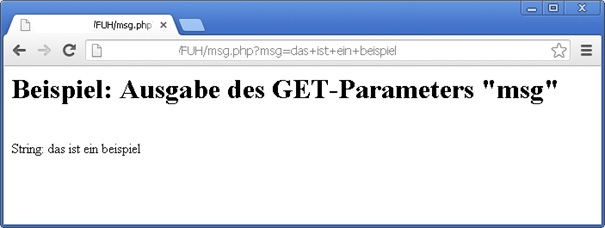
\includegraphics[scale=.75]{abbildungen/xss_1}
 \caption{Ausgabe des Beispiel-Strings}
 \label{fig:xss_1} 
\end{figure}

\begin{figure}[htbp]
 \centering
 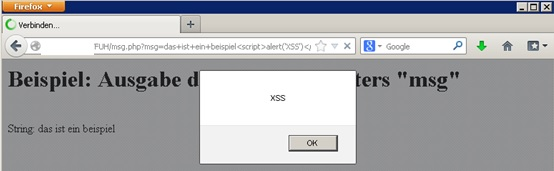
\includegraphics[scale=.75]{abbildungen/xss_2}
 \caption{Der JavaScript-Code kommt im Browser zu Ausführung}
 \label{fig:xss_2} 
\end{figure}

\newpage
Betrachtet man den Quellcode von Abbildung \ref{fig:xss_2}, so 
erkennt man den in HTML eingebetteten JavaScript-Code:

\begin{lstlisting}[basicstyle=\ttfamily\footnotesize]
<html>
  <body>
    <h1>Beispiel: Ausgabe des GET-Parameters "msg"</h1>
    <br>
    String: das ist ein beispiel
    <script>alert('XSS')</script>
  </body>
</html>
\end{lstlisting}

\subsection{Maßnahmen zur Behebung von Cross-Site-Scripting-Schwachstellen}
	
In diesem Abschnitt werden mögliche Maßnahmen zur Behebung von 
Cross-Site-Scripting-Schwachstellen vorgestellt.

\subsubsection{Encoding von HTML-Metazeichen}
	
Durch HTML-Encoding\footnote{\url{http://en.wikipedia.org/wiki/Character\_encodings\_in\_HTML}} 
werden bestimmte HTML-Metazeichen auf äquivalente Zeichenfolgen abgebildet.

Beim Aufruf der URL aus dem Beispiel würde der Wert des Parameters 
\texttt{msg} wie folgt encodiert und im Quelltext dargestellt werden:

\begin{lstlisting}[basicstyle=\ttfamily\footnotesize]
<html>
  <body>
    <h1>Beispiel: Ausgabe des GET-Parameters "msg"</h1>
    <br>
    String: das ist ein beispiel
    &lt;script&gt;alert(&#39;XSS&#39;)&lt;/script&gt;
  </body>
</html>
\end{lstlisting}

Wie der Ausgabe zu entnehmen ist, wurden die typischen HTML-Metazeichen 
serverseitig encodiert und werden aus diesem Grund vom Browser nicht 
mehr als HTML-Metazeichen interpretiert. Der Versuch, eine JavaScript-Messagebox 
mit dem Inhalt "XSS" aufpoppen zu lassen schlug fehl.

\subsubsection{HMTL-Tag-Filter}

Bei manchen Systemen (z.B. bei Diskussionsforen) ist ein vollständiges 
HTML-Encoding nicht möglich, da für die Erstellung von Beiträgen 
möglicherweise HTML-Markup benötigt wird. 

Dabei ist das Vorgehen bei der Verwendung von Tag-Filtern ähnlich der 
empfohlenen Maßnahmen zur Behebung von Injection-Schwachstellen 
(siehe Abschnitt \ref{escpace_metazeichen}), bei denen ein Filter auf 
nicht benötigte Zeichen- und Zeichenketten matchen muss. Es ist 
beispielsweise nicht davon auszugehen, dass innerhalb eines 
Diskussionsforums absichtlich ein JavaScript-Tag eingefügt werden 
muss. Aus diesem Grund kann auf den Tag \texttt{<script>} verzichtet 
werden. Ebenso sollte der Filter Schlüsselwörter erkennen, die unter 
Umständen zur Ausführung von JavaScript-Code führen, wie z.B:

\begin{lstlisting}[basicstyle=\ttfamily\footnotesize]
<style type="text/javascript">alert('XSS')</sytle>
\end{lstlisting}

An dieser Stelle sei darauf hingewiesen, dass bei der Verwendung von 
Tag-Filtern (bzw. Blacklist-Filtern) nach Möglichkeit auf eine 
eigenständige Implementierung verzichtet werden sollte und auf 
"Best-Practice"-Lösungen wie beispielsweise die OWASP 
ESAPI-Bibliothek zurückgegriffen werden sollte.

Dabei ist weiterhin zu beachten, dass sich die kritischen HTML-Tags 
zwischen den verschiedenen HTML-Versionen unterscheiden können. 
Durch die Einführung von HTML-5 können beispielsweise Filter, die 
lediglich auf für HTML-4.x relevante Zeichen- und Zeichenketten 
matchen umgangen werden. Eine ausführliche Beschreibung der 
verschiedensten Umgehungsmöglichkeiten von HTML-4-Filtern durch 
HTML-5-Tags sind im HTML-5-Cheat-Sheet\footnote{\url{http://html5sec.org/}} 
zu finden.

\subsubsection{Verwendung des Model-View-Controller-Pattern}

Im Regelfall benötigt die eigentliche Anwendungslogik keine Details 
über die spätere Darstellung der Informationen. Das bedeutet, dass 
Eingabeparameter auf ihre erwarteten Werte reduziert werden können 
ohne Zusatzinformationen über beispielsweise ihre Darstellung beinhalten 
zu müssen.

Aus diesem Grund kann man bereits bei der Entwicklung von Anwendungen 
nach dem Model-View-Controler (MVC) Entwicklungspattern vorgehen. Dabei 
werden die Daten (Model), die Darstellung (View) und die 
Benutzerinteraktionen (Controller) strikt voneinander getrennt. 
Benutzereingaben werden auf diese Weise strikt von ihrer späteren 
(erneuten) Darstellung während der Ausgabe getrennt.

Wird dieses MVC-Konzept konsequent bei der Anwendungsentwicklung 
fortgeführt, reduziert sich das Risiko von Cross-Site-Scripting-Schwachstellen 
aufgrund der konsequenten Trennung von Daten und deren Darstellung.


\newpage
\subsection{Buffer-Overflow-Schwachstellen}	

Buffer-Overflow-Schwachstellen entstehen im Regelfall durch die 
Verwendung von Programmiersprachen, die es einem Entwickler ermöglichen, 
allozierte Speicherbereiche unkontrolliert zu überschreiben.

\par\medskip 
Als ein typischer Vertreter für eine Programmiersprache, die potenziell 
für Buffer-Schwachstellen anfällig ist, gilt die Programmiersprache C. 
Diese Programmiersprache ermöglicht es einem Entwickler, nahezu beliebige 
Speicheradressen zu überschreiben und bietet darüber hinaus noch 
zahlreiche eigene, native C-Funktionen (z.B. \texttt{strcpy()}), die 
unabhängig vom Entwickler keinerlei Prüfungen in Hinsicht auf den 
benötigten Speicherplatz implementiert haben.
\\\\
\textbf{Beispiel: Stack-Overflow (Setup: x64-System, Linux, gcc-4.8.1)}
\\
Der C-Code im folgenden Beispiel erwartet die Eingabe einer beliebigen 
Zeichenkette mit einer maximalen Länge von 63 Zeichen zzgl. 
des String-Ende-Zeichens als Kommandozeilenparameter. 
Die im Code verwendete C-Funktion \texttt{strcpy()} gilt als unsicher, 
da keine Längenprüfung des zu kopierenden Strings vorgenommen wird. 
Mithilfe der \texttt{strcpy()}-Funktion ist es später möglich, die 
Rücksprungadresse der \texttt{go()}-Funktion so zu modifizieren, dass 
die im Code nicht aufgerufene Funktion \texttt{pwnd()} ausgeführt wird.

\begin{lstlisting}[basicstyle=\ttfamily\footnotesize]
#include <string.h>
#include <stdlib.h>
#include <stdio.h>

int go(char *input) {
        char data[64];
        strcpy(data,input);
        printf ("String: %s\n", data);
        return 1;
}

void pwnd(void) {
        printf("\nPWND!\n");
        exit(0);
}

int main(int argc, char *argv[]) {
        if (argc > 1)
        go(argv[1]);
}
\end{lstlisting}

\begin{figure}[htbp]
 \centering
 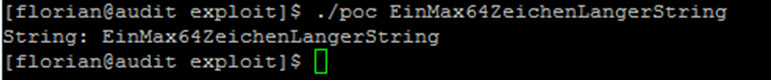
\includegraphics[scale=.5]{abbildungen/poc_1}
 \caption{Reguläre Funktionsweise des Programms}
 \label{fig:poc_1} 
\end{figure}

\newpage
Im Folgenden wird das Programm analysiert und versucht, durch eine erfolgreiche Modifikation der Speicheradressen die Funktion \texttt{pwnd()} aufzurufen.
Um das Programm zu analysieren, wird der GNU Debugger\footnote{\url{http://www.gnu.org/software/gdb}} 
(GDB-Kurzreferenz\footnote{\url{http://beej.us/guide/bggdb}}) verwendet. 
Für einen ersten Überblick werden die drei Funktionen disassembliert.
\\
\\
\texttt{main()}-Funktion
\begin{lstlisting}[basicstyle=\ttfamily\footnotesize]
[user@audit exploit]$ gdb -q poc
Reading symbols from /home/user/exploit/poc...done.
(gdb) disas main
Dump of assembler code for function main:
   0x0000000000400624 <+0>:     push   %rbp
   [...]
   0x000000000040063d <+25>:    add    $0x8,%rax
   0x0000000000400641 <+29>:    mov    (%rax),%rax
   0x0000000000400644 <+32>:    mov    %rax,%rdi
   0x0000000000400647 <+35>:    callq  0x4005d0 <go>
   0x000000000040064c <+40>:    leaveq
   0x000000000040064d <+41>:    retq
End of assembler dump.
\end{lstlisting}


\texttt{go()}-Funktion
\begin{lstlisting}[basicstyle=\ttfamily\footnotesize]
(gdb) disas go
Dump of assembler code for function go:
   [...]
   0x00000000004005e0 <+16>:    lea    -0x40(%rbp),%rax
   0x00000000004005e4 <+20>:    mov    %rdx,%rsi
   0x00000000004005e7 <+23>:    mov    %rax,%rdi
   0x00000000004005ea <+26>:    callq  0x400480 <strcpy@plt>
   0x00000000004005ef <+31>:    lea    -0x40(%rbp),%rax
   0x00000000004005f3 <+35>:    mov    %rax,%rsi
   0x00000000004005f6 <+38>:    mov    $0x4006d4,%edi
   0x00000000004005fb <+43>:    mov    $0x0,%eax
   0x0000000000400600 <+48>:    callq  0x4004a0 <printf@plt>
   0x0000000000400605 <+53>:    mov    $0x1,%eax
   0x000000000040060a <+58>:    leaveq
   0x000000000040060b <+59>:    retq
End of assembler dump.
\end{lstlisting}

\newpage
\texttt{pwnd()}-Funktion
\begin{lstlisting}[basicstyle=\ttfamily\footnotesize]
(gdb) disas pwnd
Dump of assembler code for function pwnd:
   0x000000000040060c <+0>:     push   %rbp
   [...]
\end{lstlisting}
\par\medskip 
Aus den disassemblierten Funktionen können folgende Informationen entnommen werden:
\\
\textbf{\texttt{main()}-Funktion}

\begin{itemize}
      \item \texttt{0x0000000000400647 <+35>:    callq  0x4005d0 <go>}\\
        An dieser Stelle wird durch einen \texttt{call} die Funktion \texttt{go()} aufgerufen.
      \item \texttt{0x000000000040064c <+40>:    leaveq}\\
        Wurde die \texttt{go()}-Funktion erfolgreich durchlaufen, wird aus der \texttt{go()}-Funktion an diese Speicheradresse in die \texttt{main()}-Funktion zurückgesprungen.       
\end{itemize}
\textbf{\texttt{go()}-Funktion}

\begin{itemize}
      \item \texttt{x00000000004005ef <+31>:    lea    -0x40	(\%rbp), \%rax}\\
        Aufgrund des vorhandenen C-Codes ist bereits bekannt, dass für die \texttt{strcpy()}-Funktion ein \SI{64}{Byte} großes Charakter-Array (\texttt{char data[64]}) als Ziel des Kopiervorgangs reserviert wurde. Läge der C-Code nicht vor, könnte man durch den hexadezimalen Wert \texttt{0x40} die maximale Speichergröße von \SI{64}{Byte} feststellen.        
      \item \texttt{0x000000000040060b <+59>:    retq}\\
        Nach der Ausführung dieser Instruktion muss der Befehlszeiger (IP, bei x64 RIP abgekürzt) auf die Speicheradresse \texttt{0x40064c} innerhalb der \texttt{main()}-Funktion zeigen.
\end{itemize}



\textbf{\texttt{pwnd()}-Funktion}

\begin{itemize}
      \item \texttt{0x000000000040060c <+0>:     push   \%rbp}\\
        Um die \texttt{pwnd()}-Funktion aus der \texttt{pwnd()}-Funktion heraus aufrufen zu können, muss der Befehlszeiger (RIP) innerhalb der \texttt{go()}-Funktion auf die Speicheradresse \texttt{0x40060c} geändert werden. 
\end{itemize}

\newpage
Im Folgenden wird das Programm mit dem GDB gestartet, davor wird noch ein 
Haltepunkt an der Speicheradresse \texttt{0x40060b} gesetzt (siehe 
letzte Zeile der disassemblierten \texttt{go()} -Funktion), um die 
Überlegungen verifizieren zu können.
        
\begin{lstlisting}[basicstyle=\ttfamily\footnotesize]
gdb) break *0x40060b
Breakpoint 6 at 0x40060b: file poc.c, line 13.
(gdb) run AAAAAAAA

String: AAAAAAAA

Breakpoint 6, 0x000000000040060b in go 
(input=0x7fffffffecdb "AAAAAAAA") at poc.c:13}

(gdb) p &data
$20 = (char (*)[64]) 0x7fffffffe950
(gdb) x/12xg 0x7fffffffe950
0x7fffffffe950: 0x4141414141414141      0x00007ffff7ff9100
0x7fffffffe960: 0x00007ffff7ffe190      0x0000000000f0b2ff
0x7fffffffe970: 0x0000000000000001      0x000000000040069d
0x7fffffffe980: 0x00007fffffffe9be      0x0000000000000000
0x7fffffffe990: 0x00007fffffffe9b0      0x000000000040064c
0x7fffffffe9a0: 0x00007fffffffea98      0x0000000200000000
(gdb)
\end{lstlisting}

Das Programm wird mit 8-mal "A" als Konsolenparameter gestartet. Ist der Haltepunkt erreicht, wird der \SI{64}{Byte} große Speicherbereich der Variablen \texttt{data} gesucht. Im Anschluss werden vom Beginn des Speicherbereichs der Variablen \texttt{data} 12-mal \SI{8}{Byte} große Speicherbereiche dargestellt. 

Die ersten \SI{8}{Byte} entsprechen der hexadezimalen Darstellung der Zeichenfolge \texttt{AAAAAAAA}, die als Übergabeparameter verwendet wurde. Die folgenden 7-mal \SI{8}{Byte} großen Speicherblöcke werden nicht verwendet und beinhalten ausschließlich zufällige Werte. Um die Rücksprungadresse erfolgreich zu modifizieren, sind die folgenden \SI{8}{Byte} bzw. \SI{16}{Byte} relevant:

\begin{lstlisting}[basicstyle=\ttfamily\footnotesize]
0x7fffffffe990: 0x00007fffffffe9b0      0x000000000040064c
\end{lstlisting}

Der linke Teil entspricht dem Basepointer (RBP), der rechte Teil entspricht 
der Rücksprungadresse in die \texttt{main()}-Funktion. Wird diese Adresse 
mit der Speicheradresse der \texttt{pwnd()}-Funktion überschrieben, so 
springt das Programm zur Laufzeit in die \texttt{pwnd()}-Funktion und 
führt diese aus.
 
\newpage 
Mit den folgenden Befehlen wird die \texttt{go()}-Funktion disassembliert, 
um den Startwert der \texttt{go()}-Funktion festzustellen. Im Anschluss 
werden die 12-mal \SI{8}{Byte} großen Speicheradressen 
ausgegeben und  \SI{2}{Byte} der Rücksprungadresse \texttt{0x40064c} modifiziert. 
Danach wird das Programm weiter ausgeführt und springt in die 
\texttt{pwnd()}-Funktion.

\begin{lstlisting}[basicstyle=\ttfamily\footnotesize]
(gdb) disas pwnd
Dump of assembler code for function pwnd:
   0x000000000040060c <+0>:     push   %rbp
   [...]	

End of assembler dump.
(gdb) x/12xg 0x7fffffffe950
0x7fffffffe950: 0x4141414141414141      0x00007ffff7ff9100
0x7fffffffe960: 0x00007ffff7ffe190      0x0000000000f0b2ff
0x7fffffffe970: 0x0000000000000001      0x000000000040069d
0x7fffffffe980: 0x00007fffffffe9be      0x0000000000000000
0x7fffffffe990: 0x00007fffffffe9b0      0x000000000040064c
0x7fffffffe9a0: 0x00007fffffffea98      0x0000000200000000
(gdb) set {char}0x7fffffffe998 = 0x0c
(gdb) set {char}0x7fffffffe999 = 0x06
(gdb) x/12xg 0x7fffffffe950
0x7fffffffe950: 0x4141414141414141      0x00007ffff7ff9100
0x7fffffffe960: 0x00007ffff7ffe190      0x0000000000f0b2ff
0x7fffffffe970: 0x0000000000000001      0x000000000040069d
0x7fffffffe980: 0x00007fffffffe9be      0x0000000000000000
0x7fffffffe990: 0x00007fffffffe9b0      0x000000000040060c
0x7fffffffe9a0: 0x00007fffffffea98      0x0000000200000000
(gdb) c
Continuing.
PWND!
[Inferior 1 (process 1190) exited normally]
(gdb)
\end{lstlisting}

Um den Aufwand einer manuellen Modifikation der Speicheradresse 
möglichst gering zu halten, kann man den Vorgang mit der Script-Sprache \texttt{Perl} 
automatisieren:

\begin{lstlisting}[basicstyle=\ttfamily\footnotesize]
(gdb) run `perl -e 'print "A"x72 . "\x0c\x06\x40"'`
String: AAAAAAAAAAAAAAAAAAAAAAAAA ... AAAAAA@
PWND!
[Inferior 1 (process 1624) exited normally]
(gdb)
\end{lstlisting}

\newpage
Dabei werden insgesamt \SI{72}{Byte} mit dem Zeichen \texttt{A} 
überschrieben und \SI{3}{Byte} mit hexadezimalen Werten:

\begin{itemize}
      \item \SI{64}{Byte} Speicherplatz der \texttt{data}-Variablen    
      \item \SI{8}{Byte} Basepointer
      \item \SI{3}{Byte} Rücksprungadresse unter Berücksichtigung der Byteorder (Little-Endian)
\end{itemize}

\textbf{Hinweis:}

Wird zur Nachstellung des Beispiels ein veralteter \texttt{gcc}-Compiler 
in der Version 3.x\footnote{\url{http://www.trapkit.de/papers/gcc\_stack\_layout\_v1\_20030830.pdf}} 
verwendet, ist es möglich, dass dieses Beispiel nicht funktioniert!

\subsection{Maßnahmen zur Behebung von Overflow-Schwachstellen}

In den folgenden Abschnitten werden Möglichkeiten beschrieben, wie man 
typische Overflow-Schwachstellen innerhalb eines Quelltextes aufspüren 
und beheben kann. Die folgend gezeigten Beispiele beziehen sich auf das 
im vorhergehenden Abschnitt beschriebe Quellcodebeispiel.

\subsubsection{Lexikalische Quellcode-Überprüfung}

Für eine lexikalische Überprüfung des Quellcodes können eine Vielzahl 
von Tools eingesetzt werden. Die Methoden reichen dabei von einer 
rudimentären grep-Analyse, über komplexe und meist kommerzielle 
statische Quellcodescanner-Lösungen (z.B. Fortify oder Checkmarx) 
bis hin zu Lösungen, die den Quellcode einer Anwendung sowohl statisch 
analysieren und zur Ausführung bringen um Laufzeitfehler erkennen zu 
können (z.B. Seeker)
Eine Liste von potentiell unsicheren C-Funktionen und deren "sicheren" 
Derivate sind in den folgenden beiden, vom ISO-Komitee herausgegeben, 
Dokumenten zu finden:

\begin{itemize}
      \item TR 24731-1\footnote{\url{http://www.open-std.org/JTC1/SC22/WG14/www/docs/n1225.pdf}}   
      \item TR 24731-2\footnote{\url{http://www.open-std.org/JTC1/SC22/WG14/www/docs/n1337.pdf}}
\end{itemize}
	
Die beiden Dokumente werden in Foren und Fachkreisen kontrovers 
diskutiert, dennoch ist das Dokument TR 24731-1 in die Entwicklung 
der Microsoft-Standard-C Bibliothek eingeflossen. Weiterhin wurden 
Empfehlungen aus den Dokumenten, wie z.B. die Entfernung der im 
C99-Standard noch enthaltenen \texttt{gets()}-Funktion, im neuen 
C-Standard (C11) umgesetzt.
Im Folgenden sollen nur zwei Beispiele für eine lexikalische Suche 
nach unsicheren Funktionen am Quellcode aus dem vorhergehenden 
Abschnitt hergenommen werden:
\par\medskip 
Durch \texttt{grep()} werden sämtliche Zeilen des Quellcodebeispiels 
ausgegeben, in denen die Funktionen \texttt{strcpy()} und \texttt{gets()} 
aufgerufen werden. Bei diesem Vorgehen obliegt es dem Entwickler, diese 
Stellen im Quellcode eingehend auf Schwachstellen zu untersuchen und 
die unsicheren Funktionen durch die empfohlen Funktionsderivate zu 
ersetzen.

\begin{lstlisting}[basicstyle=\ttfamily\footnotesize]
[user@audit exploit]$ grep -nE 'strcpy|gets' *.c
poc.c:9:        strcpy(data,input);
\end{lstlisting}

Es ist abzusehen, dass bei umfangreichen Quelltextanalysen eine solch 
rudimentäre Analyse zu einer sehr hohen "False-Postives"-Rate führt. 
Aufgrund dieser Tatsache wurden lexikalische Quellcodescanner mit dem 
Ziel entwickelt, die Effizienz der Methode zu verbessern.

Effiziente Quellcodescanner reduzieren die Rate der gefundenen 
"False-Postives" beispielsweise durch die Verwendung interner 
Datenbanken, die  potenziell unsichere Quellcodefragmente mit den in 
der Datenbank hinterlegten Codefragmenten abgleichen. Dabei wird 
weiterhin versucht, den Entwickler durch entsprechende Kommentare zu 
einer möglicherweise gefundenen Schwachstelle zu unterstützen. Ein 
Quellcodescanner sollte weder "False-Postives" noch "False-Negatives" 
produzieren. Dabei sollten "False Negatives" nach Möglichkeit nie 
vorkommen, da diese im Gegensatz zu "False Positives" zu 
Sicherheitsproblemen führen können.

Nachfolgend soll der frei verfügbare Quellcodescanner RATS\footnote{\url{https://www.fortify.com/downloads2/public/rats-2.3-2.tar.gz}} 
(Rough Auditing Tool for Security) vorgestellt werden. RATS ist in der 
Lage, C-, C++-, PHP-, Perl- und Python-Quelltext nach 
sicherheitsrelevanten Fehlern zu untersuchen. Schwerpunktmäßig 
berücksichtigt RATS dabei Buffer-Overflow- und Race-Condition-Schwachstellen.

\begin{lstlisting}[basicstyle=\ttfamily\footnotesize]
[user@audit exploit]$ rats -i --resultsonly  *.c
poc.c:8: High: fixed size local buffer
Extra care should be taken to ensure that character arrays that 
are allocated on the stack are used safely.  They are prime 
targets for buffer overflow attacks.

poc.c:9: High: strcpy
Check to be sure that argument 2 passed to this function 
call will not copy more data than can be handled, resulting 
in a buffer overflow.
\end{lstlisting}

Bei der Ausgabe von RATS wird ein Nutzer gleich zu Beginn auf die 
Verwendung von Variablen mit fixer Puffergröße aufmerksam gemacht. 
Darüber hinaus wird darauf hingewiesen, dass man diese Puffer in 
Bezug auf potenzielle Buffer-Overflow-Schwachstellen überprüfen sollte.

Im weiteren Verlauf der Ausgabe wird auf die Verwendung der 
unsicheren \texttt{strcpy()}-Funktion und auf deren sichere 
Implementierung unter Berücksichtigung der benötigten Speichergröße 
des Zielpuffers hingewiesen.

\subsubsection{Semantische Quellcode-Überprüfungen}

Es existiert neben der rein lexikalischen Quelltextanalyse ein weiteres 
Analyseverfahren zur statischen Codeanalyse. Eine semantische 
Quellcode-Analyse erlaubt es, die lexikalischen Bedeutungen innerhalb des 
Quelltextes in Bezug auf ihren Bedeutungszusammenhang auszuwerten. 
Dabei bedient sich diese Analysemethode einer Datenflussanalyse und ist 
somit in der Lage, detaillierte Rückschlüsse über laufende Vorgänge 
innerhalb eines Programms zuzulassen.

\minisec{Grundlegende Überprüfungen mit dem Compiler}

Ein Compiler verfügt bereits meist über grundlegende Techniken, 
um mindestens eine lexikalische und zusätzlich eine semantische Analyse 
des Quellcodes durchzuführen. Der GNU C Compiler verfügt über verschiedene 
Optionen, die eine Fehlervermeidung oder eine Fehlersuche unterstützen.

Wird bei Aufruf des GNU C Compilers die Option \texttt{–Wall} angegeben, 
veranlasst dies den Compiler dazu, eine Überprüfung des Quelltextes 
während des Kompilierens durchzuführen. Um die Meldungen des Compilers 
offensichtlicher zu gestalten, wird die \texttt{main()}-Funktion durch 
die folgenden Codezeilen ergänzt:

\begin{lstlisting}[basicstyle=\ttfamily\footnotesize]
int main(int argc, char *argv[]) {
    [...]
    char array[8];
    printf("String eingeben: ");
    gets(array);
    printf ("Input-String: %s", array);
}
\end{lstlisting}

Wird der Quellcode jetzt mit der – Wall-Funktion kompiliert, erhält man 
folgende Compiler-Warnungen:

\begin{lstlisting}[basicstyle=\ttfamily\footnotesize]
[user@audit exploit]$ gcc -Wall poc.c -o poc
poc.c: In function main:
poc.c:29:2: warning: gets is deprecated 
(declared at /usr/include/stdio.h:638) [-Wdeprecated-declarations]
  gets(array);
poc.c:31:1: warning: control reaches end of non-void 
function [-Wreturn-type]
}
\end{lstlisting}

Der GNU C Compiler macht den Entwickler darauf aufmerksam, dass er zum 
einen die unsichere und veraltete \texttt{gets()}-Funktion verwendet und 
zum anderen, dass die \texttt{main()}-Funktion über keinen Return-Wert am 
Ende verfügt.

Anhand dieses Beispiels ist ersichtlich, dass der Compiler zwar in der 
Lage ist, Sicherheitsüberprüfungen auf lexikalischer und semantischer 
Ebene durchzuführen, jedoch offensichtlich nicht dazu in der Lage ist, 
unsichere Funktionsaufrufe wie z.B. den Aufruf der \texttt{strcpy()}-Funktion 
innerhalb der \texttt{go()}-Funktion zu erkennen.

\minisec{Erweiterte Überprüfung mit Splint}

Splint\footnote{\url{http://www.splint.org/}} ist ein statischer Quellcodescanner, 
der in der Lage ist, eine weitaus detaillierte semantische Analyse als 
der GNU C Compiler vorzunehmen.

Splint ist imstande, sogenannte LINT\footnote{\url{http://en.wikipedia.org/wiki/Lint\_(software)}}-Überprüfungen 
durchzuführen. Zu diesen Überprüfungen gehören beispielsweise die Suche 
nach Endlosschleifen, falschen Deklarationen oder ignorierten Rückgabewerten.

Im folgenden Beispiel wird der Beispielquelltext durch die Angabe des 
Parameters \texttt{+bounds-write} auf potenzielle Schwachstellen hin 
untersucht, die aufgrund eines schreibenden Speicherzugriffs zu einem 
Buffer-Overflow führen können.

\begin{lstlisting}[basicstyle=\ttfamily\footnotesize]
[user@audit exploit]$ splint +bounds-write poc.c
Splint 3.1.2 --- 14 Sep 2011

poc.c: (in function go)
poc.c:9:2: Possible out-of-bounds store: strcpy(data, input)
    Unable to resolve constraint:
    requires maxRead(input @ poc.c:9:14) <= 63
     needed to satisfy precondition:
    requires maxSet(data @ poc.c:9:9) >= maxRead
    (input @ poc.c:9:14)
     derived from strcpy precondition: requires maxSet
     (<parameter 1>) >=
    maxRead(<parameter 2>)
  A memory write may write to an address beyond the 
  allocated buffer. (Use -boundswrite to inhibit warning)
poc.c: (in function main)
poc.c:25:2: Return value (type int) ignored: go(argv[1])
  Result returned by function call is not used. If this is 
  intended, can cast result to (void) to eliminate message. 
  (Use -retvalint to inhibit warning)
  [...]
\end{lstlisting}

Der Scanner erkennt im Gegensatz zum GNU C Compiler, dass es durch den 
Aufruf der \texttt{strcpy()}-Funktion zu einem möglichen Speicherüberlauf 
kommen könnte. Durch die Verwendung von Annotationen innerhalb des zu 
prüfenden Quellcodes können vom Entwickler neben programmatischen Fehlern 
auch logische Fehler entdeckt werden. Beispielsweise können durch  
Annotationen zwingend zu erfüllende Bedingungen festgelegt werden, 
die durch Splint geprüft werden, bevor eine bestimmte Funktion aufgerufen 
werden kann.

\subsubsection{Programmanalyse zur Programmlaufzeit}

Neben den beschreiben Möglichkeiten zur statischen Quellcodeanalyse 
besteht darüber hinaus die Möglichkeit, ein Programm zur Laufzeit auf 
Schwachstellen zu überwachen bzw. zu untersuchen, um gezielt 
Overflow-Schwachstellen, die erst zur Programmlaufzeit entstehen 
ausfindig zu machen.

Ein mögliches Beispiel für eine potenzielle Overflow-Schwachstelle, die 
erst während der Laufzeit eines Programmes auftreten kann, ist der 
Aufruf der C-Funktion \texttt{malloc()}, die Speicher im Heap alloziert.

Ein typisches Tool zur Programmanalyse zur Laufzeit ist ein Debugger. 
Mit einem Debugger kann man Programme zeilenweise abarbeiten und dabei 
den aktuellen Zustand bzw. den Wert von Variablen analysieren. Die Qualität 
der Überprüfung des Programmcodes unter Zuhilfenahme eines Debuggers 
hängt stark von der Fachexpertise eines Entwicklers ab. Für die umfangreiche 
Analyse von Programmen eignet sich ein Debugger nur bedingt.

Aus diesem Grund existieren spezielle Tools, die zur dynamischen Analyse 
von umfangreicheren Programmen oder Quelltexten eingesetzt werden können. 
Im Folgenden soll die Werkzeugsammlung Valgrind vorgestellt werden.

\minisec{Programmanalyse zur Laufzeit mit Valgrind}

Valgrind stellt eine Werkzeugsammlung zur Programmlaufzeit dar, die 
dynamischen Fehleranalyse durchführt. Dabei wird ein zu analysierendes 
Programm nicht auf der nativen Host-CPU, sondern innerhalb einer 
virtuellen Umgebung ausgeführt.
Vagrind übersetzt das Programm zu diesem Zweck in einen 
plattformunabhängigen Byte-Code, in den sogenannten Vex IR. Nach der 
Konvertierung des Programms in den Byte-Code können die verschiedenen 
Valgrind-Tools auf das zu analysierende Programm angewendet werden.

Die Konvertierung des nativen Programms nach Vex IR reduziert die 
Ausführungsgeschwindigkeit eines Programmes um ein Vielfaches, 
ermöglicht aber gleichzeitig eine detaillierte Analyse  benötigter 
(Speicher-)Ressourcen oder einzelner CPU-Register.

Für das folgende Beispiel wird die \texttt{go()}-Funktion um 2 
\texttt{malloc()}-Funktionsaufrufe erweitert:

\begin{lstlisting}[basicstyle=\ttfamily\footnotesize]
int go(char *input) {
    char *data;	
    data  = (char *)malloc(sizeof(char)*8);
    data = (char *)malloc(sizeof(char)*64);

    strcpy(data,input);
    [...]
}
\end{lstlisting}

Anschließend wird das Programm kompiliert und mit Valgrind aufgerufen, 
als Startparameter wird 84-mal der Buchstabe A übergeben. Dabei kommt 
es, wie aus den vorhergehen Beispielen bereits bekannt, zu einem 
Buffer-Overflow:

\begin{lstlisting}[basicstyle=\ttfamily\footnotesize]
valgrind --tool=memcheck --leak-check=full 
./poc `perl -e 'print "A"x84'`
\end{lstlisting}

Valgrind überprüft nun das Programm \texttt{poc} zur Laufzeit und 
generiert folgende Ausgabe:

\begin{lstlisting}[basicstyle=\ttfamily\footnotesize]
[...]
==10902== Invalid write of size 1
==10902== at 0x4C2CBB2: __GI_strcpy 
          (in /usr/lib/valgrind/vgpreload_memcheck- 
          amd64-linux.so)
==10902== by 0x40069A: go (poc2.c:14)
==10902== by 0x400703: main (poc2.c:31)
==10902== Address 0x51e00e4 is 20 bytes after a block 
          of size 64 alloc'd
==10902== at 0x4C2C04B: malloc 
          (in /usr/lib/valgrind/vgpreload_memcheck- 
          amd64-linux.so)
[...]
==10902== HEAP SUMMARY:
==10902== in use at exit: 8 bytes in 1 blocks
==10902== total heap usage: 2 allocs, 1 frees, 72 bytes 
          allocated
==10902==
==10902== 8 bytes in 1 blocks are definitely lost in loss 
		  record 1 of 1
==10902== at 0x4C2C04B: malloc 
          (in /usr/lib/valgrind/vgpreload_memcheck-
          amd64-linux.so)
==10902== by 0x400675: go (poc2.c:9)
==10902== by 0x400703: main (poc2.c:31)
[...]
\end{lstlisting}

Wie der Ausgabe zu entnehmen ist, erkennt Valgrind zum einen, dass es 
beim Aufruf der \texttt{strcpy()}-Funktion zu einem Überlauf von \SI{20}{Byte} 
kommt und zum anderen, dass der \SI{8}{Byte} große (reservierte) 
Speicherblock aufgrund der fehlenden \texttt{free()}-Funktion nicht mehr 
freigeben wird und es zu einem unnötigen Verbrauch von Heap-Speicher kommt.



%%%%%%%%%%%%%%%%% Kapitel 4 %%%%%%%%%%%%%%%%%% 
\newpage
\thispagestyle{fancy} 
\fancyhead[L]{} %Kopfzeile links
% Kirsten
\section{Umgang mit Sicherheitslücken}
Wie geht man mit dem Bekanntwerden von Sicherheitslücken in Software um?

Bisher wurde beschrieben, welche Arten von Sicherheitslücken es gibt und 
wie man Code aktuell wirkungsvoll davor schützt. Desweiteren wurden aktuelle 
Lösungswege gezeigt, um sie zu vermeiden.

In den meisten Fällen kann man bei Bekanntwerden von Sicherheitslücken
diese beseitigen und ein Update bereitstellen.
Was aber passiert mit Code, der eine Sicherheitslücke hat, die
kritisch ist, aber nicht zeitnah aktualisiert werden kann?

Aktuell gibt es zahlreiche solcher bekannten Sicherheitslücken. Der wohl 
populärste Hacker im Dienste des "Guten" war der Sicherheitsexperte 
Barnaby Jack, der zu den sogenannten \textit{white hats} zählte. Er starb 
vergangene Woche an bislang ungeklärter Ursache im Alter von 35 Jahren
\footnote{http://www.spiegel.de/netzwelt/web/hacker-barnaby-jack-in-san-francisco-gestorben-a-913380.html}. 
Kommende Woche wollte er auf einer Konferenz über die Sicherheit von 
Herzschrittmachern sprechen.
In den Medien sorgt aktuell noch ein weiterer Fall für Schlagzeilen.
Dabei geht es um geknackte Wegfahrsperrcodes
\footnote{http://www.spiegel.de/auto/aktuell/volkswagen-erwirkt-verfuegung-gegen-akademische-codeknacker-a-913462.html} 
bei den Luxusmarken der Volkswagen Gruppe (VW).
Hier wurde von VW kurzfristig eine Verfügung veranlasst, die den Wissenschaftlern
eine Veröffentlichung untersagt.

Beide Beispielfälle zeigen Sicherheitslücken in Systemen, die
nur schwer aktualisiert werden können. 
Die Softwareentwicklung bei einem Herzschrittmacher benötigt viele
Tests und einen Langzeittest um sicherzustellen, dass durch ein Update
nicht eine Fehlfunktion zum Herzstillstand des Patienten führt. 
Bei VW muss jetzt jeder betroffene Wagen in eine Werkstatt, um mit neuer
Software ausgestattet zu werden, da man nicht einfach das Update über 
eine Datenleitung einspielen kann. 
Zwar gibt es immer mehr Systeme, die eine Anbindung an das Internet haben
\footnote{http://www.n-tv.de/ratgeber/Sendungen/Wenn-nicht-nur-der-Kuehlschrank-online-ist-article10431986.html}, 
doch bringt dieses nicht nur Vorteile, da gerade die globale Erreichbarkeit
neue Sicherheitsprobleme hervorruft.  
Für Hersteller sind nicht nur die Fehlerbehebung und die Tests mit 
Kosten verbunden, sondern auch eine eventuelle Rufschädigung. So versuchen
gerade große Konzerne, die Hacker ihrer Systeme als Sicherheitsexperten 
zu gewinnen.



%%%%%%%%%%%%%%%%% Kapitel 5 %%%%%%%%%%%%%%%%%% 
\newpage
\thispagestyle{fancy} 
\fancyhead[L]{} %Kopfzeile links
% Kirsten
\section{Fazit}
Durch die globalisierte Vernetzung nimmt die Sicherheit in der 
Softwareentwicklung einen immer größeren Stellenwert ein. In den 
vergangenen Jahren ist die Komplexität mit jeder neu entstandenen 
Software gestiegen. 
\newline

%~ \textit{„Wann haben Sie zuletzt Ihren Smart-Fernseher aktualisiert?“} 
%~ \begin{flushright}
%~ Marc Rogers, US-Sicherheitsforscher
%~ \end{flushright} 
%~ \newline

Obwohl Sicherheitslücken wie SQL-Injection und Cross-Site Scripting (XSS), 
wie in dieser Hausarbeit beschrieben, schon seit Jahren bekannt sind und 
effektiv bekämpft werden können, liest man noch heute immer wieder über diese 
Schwachstellen. Inzwischen gibt es eigene Firmen, die bezahlt werden, um 
Sicherheitslücken zu finden und damit das Softwareprodukt sicherer zu 
machen. Doch durch die stetige Weiterentwicklung und neuen Möglichkeiten
entstehen wiederum neue Sicherheitslücken.
Auch wenn eine Schwachstelle behoben wurde bedeutet dieses nicht gleich, 
dass alle betroffenen Systeme von der Behebung profitieren.
Ein bekanntes Beispiel sind Content Managment Systeme, die von
Administratoren oft nur schlecht gewartet werden. So gibt es Schätzungen,
das heute nur ca. 50\% aller Wordpress-Installationen \cite{playground_wordpress} %\footnote{\url{http://playground.ebiene.de/wordpress-versionen-verteilung/}}
aktuell sind. Sicherheitsexperten gehen sogar aufgrund der stetigen
Entwicklung von Hardware und Softwarekomplexitäten davon aus, dass 
nach einem Jahr ohne Aktualisierungen eine Software hochgradig
anfällig für Schwachstellen ist.
Auch der gerne benutzte Punkt "Sicherheit durch Unbekanntheit" 
kann nicht genutzt werden. Gerade in Zeiten von Spionage untersuchen
Hacker Webseiten auf Auffälligkeiten.
 
Daher müssen sich nicht nur Entwickler mit der ständigen Weiterentwicklung 
auseinandersetzen, sondern auch die Nutzer dieser Software selbst. 
Auch wenn gleich es inzwischen viele Hilfsprogramme gibt, die nachschauen 
ob es eine neuere Version gibt, so muss schlussendlich doch auch der 
Nutzer tätig werden, um das Update durchzuführen.   



\onecolumn
% einfacher Zeilenabstand
\singlespacing
% Literaturliste soll im Inhaltsverzeichnis auftauchen
\newpage
\addcontentsline{toc}{section}{Literaturverzeichnis}
% Literaturverzeichnis anzeigen
\renewcommand\refname{Literaturverzeichnis}
\bibliography{Hauptdatei}

% Abstract
\newpage
\fancyhead[L]{Abstract} %Kopfzeile links
\section*{Zusammenfassung}


%\begin{verbatim}

%

%\end{verbatim}

\section*{Abstract}


% evtl. Anhang
\newpage
\addcontentsline{toc}{section}{Anhang}
\fancyhead[L]{Anhang} %Kopfzeile links
\subsection*{Anhang}\label{anhang}


\newpage
% Listingverzeichnis soll im Inhaltsverzeichnis auftauchen
\addcontentsline{toc}{section}{Listingverzeichnis}
\fancyhead[L]{Abbildungs- / Tabellen- / Listingverzeichnis} %Kopfzeile links
\renewcommand{\lstlistlistingname}{Listingverzeichnis}
\lstlistoflistings
%%%%


% das Abbildungsverzeichnis
\newpage
% Abbildungsverzeichnis soll im Inhaltsverzeichnis auftauchen
\addcontentsline{toc}{section}{Abbildungsverzeichnis}
\fancyhead[L]{Abbildungsverzeichnis} %Kopfzeile links
% Abbildungsverzeichnis endgueltig anzeigen
\listoffigures

% das Tabellenverzeichnis
\newpage
% Abbildungsverzeichnis soll im Inhaltsverzeichnis auftauchen
\addcontentsline{toc}{section}{Tabellenverzeichnis}
\fancyhead[L]{Tabellenverzeichnis} %Kopfzeile links
% \fancyhead[L]{Abbildungsverzeichnis / Abkürzungsverzeichnis} %Kopfzeile links
% Abbildungsverzeichnis endgueltig anzeigen
\listoftables

%%%%%%%%%%%%%%%%% Eidesstattliche Erklärung %%%%%%%%%%%%%%%%%% 
\thispagestyle{fancy} 

\thispagestyle{empty}

\begin{verbatim}

\end{verbatim}

\begin{LARGE}Eidesstattliche Erklärung zur Hausarbeit\end{LARGE}
\begin{verbatim}


\end{verbatim}
Ich versichere, die von mir vorgelegte Arbeit selbstständig verfasst zu 
haben. Alle Stellen, die wörtlich oder sinngemäß aus veröffentlichten 
oder nicht veröffentlichten Arbeiten anderer entnommen sind, habe ich 
als entnommen kenntlich gemacht. Sämtliche Quellen und Hilfsmittel, die 
ich für die Arbeit benutzt habe, sind angegeben. Die Arbeit hat mit 
gleichem Inhalt bzw. in wesentlichen Teilen noch keiner anderen 
Prüfungsbehörde vorgelegen.


\begin{displaymath}
% use packages: array
\begin{array}{ll}
Unterschrift:~~~~~~~~~~~~~~~~~~~~~~~~~~~~~~~~~~~~~~~~~~
& Ort, Datum:~~~~~~~~~~~~~~~~~~~~~~~~~~~~~~~~~~~~~~~~~~
\end{array}
\end{displaymath}

\newpage


\thispagestyle{empty}

\begin{verbatim}

\end{verbatim}

\begin{LARGE}Eidesstattliche Erklärung zur Hausarbeit\end{LARGE}
\begin{verbatim}


\end{verbatim}
Ich versichere, die von mir vorgelegte Arbeit selbstständig verfasst zu 
haben. Alle Stellen, die wörtlich oder sinngemäß aus veröffentlichten 
oder nicht veröffentlichten Arbeiten anderer entnommen sind, habe ich 
als entnommen kenntlich gemacht. Sämtliche Quellen und Hilfsmittel, die 
ich für die Arbeit benutzt habe, sind angegeben. Die Arbeit hat mit 
gleichem Inhalt bzw. in wesentlichen Teilen noch keiner anderen 
Prüfungsbehörde vorgelegen.


\begin{displaymath}
% use packages: array
\begin{array}{ll}
Unterschrift:~~~~~~~~~~~~~~~~~~~~~~~~~~~~~~~~~~~~~~~~~~
& Ort, Datum:~~~~~~~~~~~~~~~~~~~~~~~~~~~~~~~~~~~~~~~~~~
\end{array}
\end{displaymath}


\end{document}  % beendet das Schriftstueck 
